%\subsection{Treemap Visualization}

%\frame
%{
%   \frametitle{Treemap Visualization - Description}
%   \framesubtitle{Time-Slice Hierarchy}
%
%   \vfill
%   %based on img/treemap-description.svg
%   \includegraphics[width=\textwidth]{img/normal.pdf}
%}

\frame
{
   \frametitle{Treemap Visualization - Description}
   \framesubtitle{Time-Slice and Aggregated Hierarchies}

   \begin{itemize}
   \item Interaction Techniques: mouse wheel, mouse over
   \item Detailed information is available in the status bar
   \end{itemize}

   \vfill
   %based on img/treemap-description.svg
   \begin{center}
   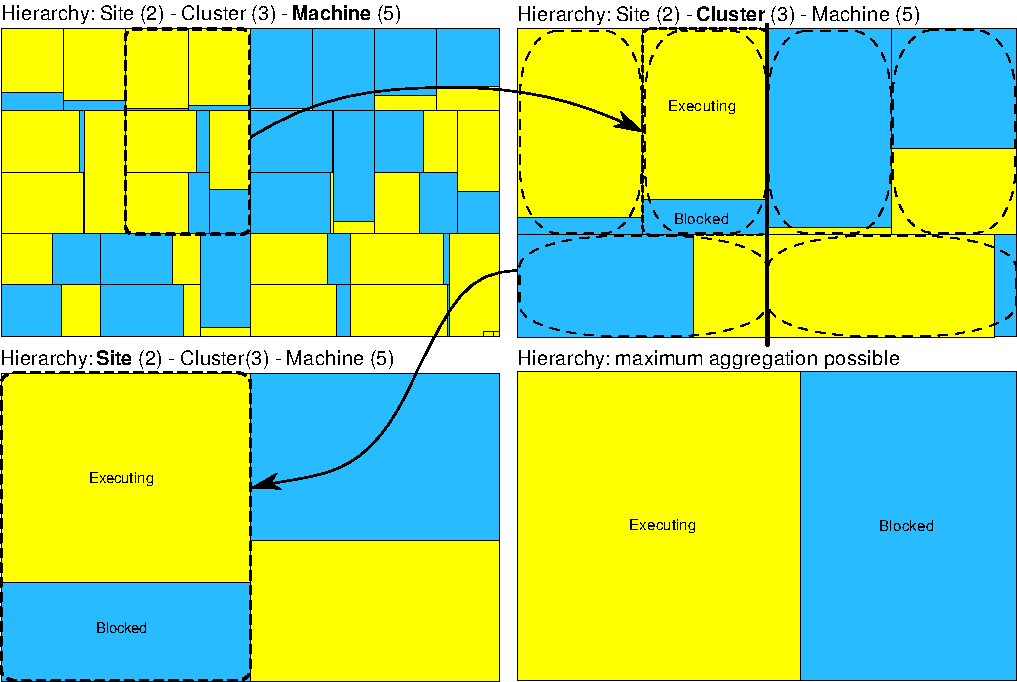
\includegraphics[width=.8\textwidth]{img/aggregated.pdf}
   \end{center}
}

\frame
{
   \frametitle{Treemap Visualization - KAAPI Trace}

%   \begin{itemize}
%   \item 2900 processes, 310 processors, four sites
%   \end{itemize}

%   \vfill
   %based on img/kaapi-scenario-c.svg
   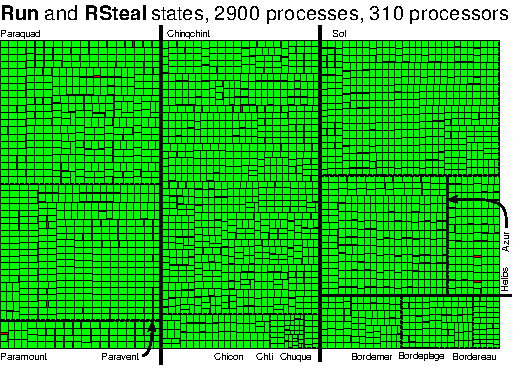
\includegraphics[width=\textwidth]{img/kaapi-scenario-c.pdf}
}


\frame
{
   \frametitle{Treemap Visualization - Large-Scale}

   \begin{itemize}
   \item Synthetic trace with 100 thousand processes
   \item Two states, four-level hierarchy
   \end{itemize}

   \vfill
   %based on img/large-scale.svg
   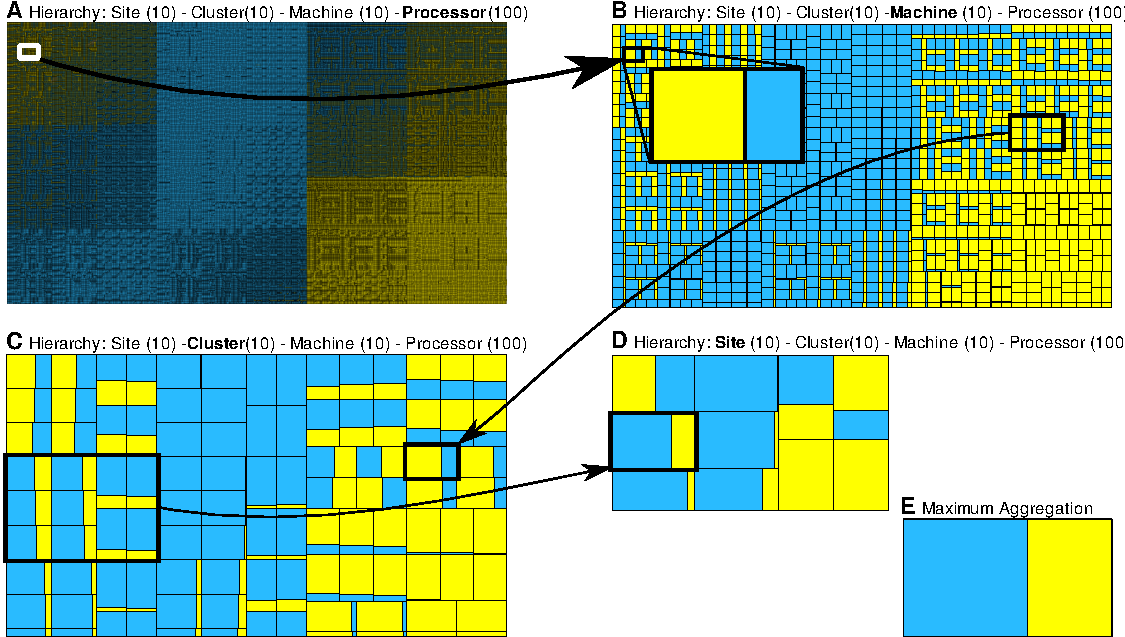
\includegraphics[width=\textwidth]{img/large-scale.pdf}
}


%\frame
%{
%   \frametitle{Treemap Visualization - KAAPI Trace}
%
%   \begin{itemize}
%   \item 200 processes, 200 machines, two sites
%   \item 100 processes per site
%   \item Different behavior: beggining/end of execution
%   \item Load-balancing between the two sites
%   \end{itemize}
%
%   \vfill
%   %based on img/kaapi-scenario-a.svg
%   \includegraphics[width=\textwidth]{img/kaapi-scenario-a.pdf}
%}


\frame
{
   \frametitle{Treemap Visualization - KAAPI Trace}

   \begin{itemize}
   \item 400 processes, 50 machines, one site
   \item 8 processes per machine
      \begin{itemize}
      \item Overload of some machines with 2 CPUs
      \item Unusual amount of time in Steal state
      \end{itemize}
   \item Machines with 4 CPUs show normal behavior
   \end{itemize}

   \vfill
   %based on img/kaapi-scenario-b.svg
   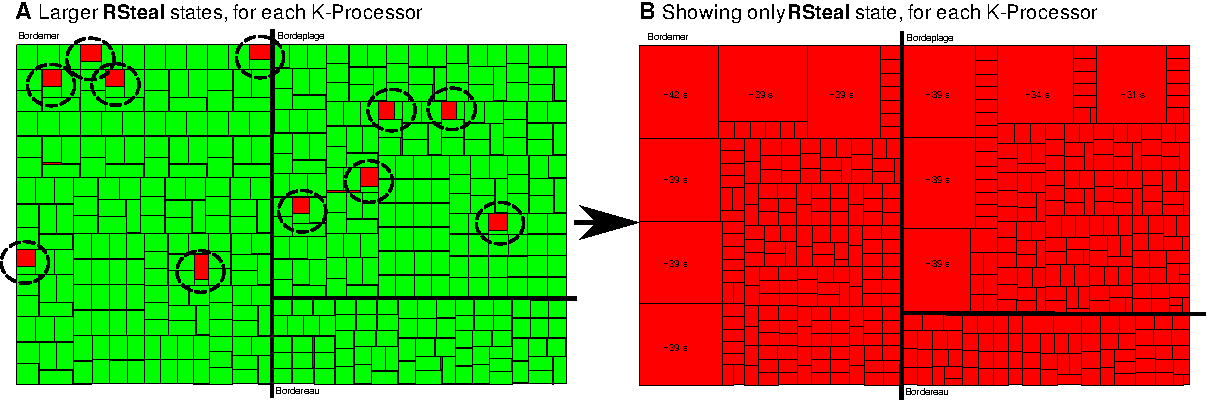
\includegraphics[width=\textwidth]{img/kaapi-scenario-b.pdf}
}

\frame
{
   \frametitle{Treemap Visualization - KAAPI Trace}

   \begin{itemize}
   \item 188 processes, 188 machines, five sites
   \item Different behavior at Porto Alegre
   \item Probably due to the interconnection
      \begin{itemize}
      \item Latency for Grid'5000 in France: \texttildelow 10 ms
      \item Latency between Porto Alegre and France: \texttildelow 300 ms
      \end{itemize}
   \item More time spent in work stealing functions
   \end{itemize}

   \vfill
   %based on img/kaapi-scenario-d.svg
   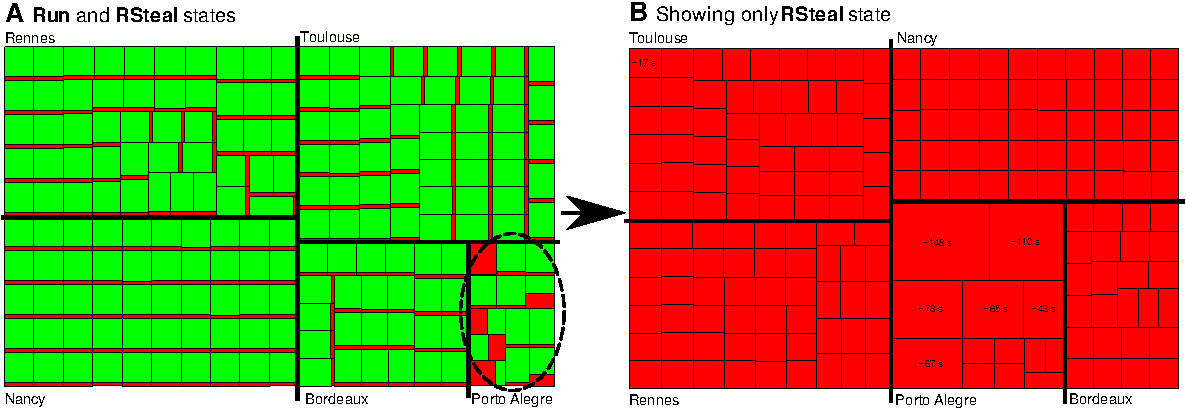
\includegraphics[width=\textwidth]{img/kaapi-scenario-d.pdf}
}

\frame
{
   \frametitle{Treemap Visualization - MPI Trace}

   \begin{itemize}
   \item Traces from the EP application -- NAS Benchmark
   \item 32 processes -- time spent in each MPI operation
   \item Init and Barrier views indicate a linear implementation
   \end{itemize}

   \vfill
   %based on img/kaapi-scenario-d.svg
   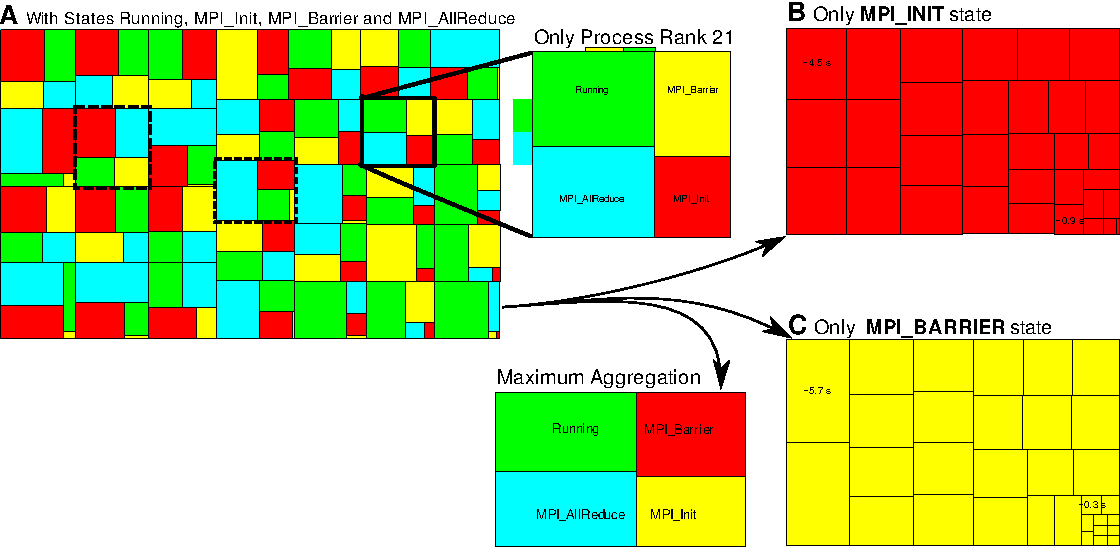
\includegraphics[width=\textwidth]{img/mpi-scenario.pdf}
}
